\documentclass[10pt]{article}
\usepackage[margin=1in]{geometry} 

\usepackage{amsmath,amsthm,amssymb,graphicx,amsfonts}

\usepackage{float}
\usepackage{caption,subcaption} % para las figuras
\usepackage{wrapfig}

\usepackage{comment}

\usepackage[utf8]{inputenc} %tildes
\usepackage[spanish]{babel}

\usepackage{enumerate}

\usepackage{color}   %May be necessary if you want to color links
\usepackage{hyperref}
\hypersetup{
	colorlinks=true, %set true if you want colored links
	linktoc=all,     %set to all if you want both sections and subsections linked
	linkcolor=blue,  %choose some color if you want links to stand out
}

\begin{document}
	
\title{Población Penitenciaria en Argentina\\ 2002 a 2017 \\
	\begin{small}
		Tutor: Franco Camporeale
	\end{small}}
\author{\small{Nahuel Almeida, María Lucía Pappaterra, Javier ¿?}}

\maketitle

\section{Análisis estadístico de variables}

Seleccionar un conjunto de al menos cuatro variables que resulten de interés.

\begin{enumerate}
	\item Usar distintos tipos de gráficos para describir sus distribuciones
	\item Analizar Outliers
	\item Calcular estadísticos clásicos (media, mediana, moda, desviación estandar)
\end{enumerate}

Las variables elegidas fueron: edad, duración de condena, 

\subsection{Edad}

\begin{figure}[H]
	\centering
	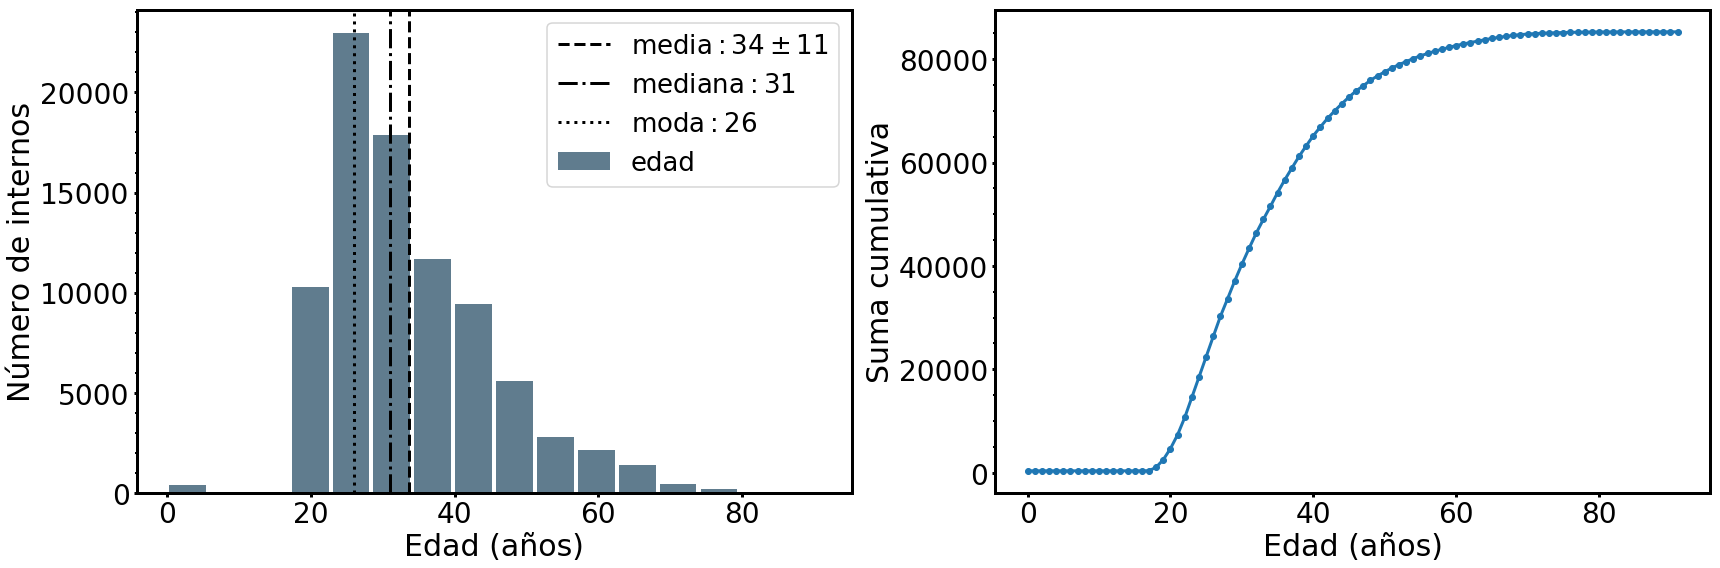
\includegraphics[scale=0.3]{graficos/edad.png}
	\caption{}
\end{figure}

\subsection{Duración de condena}

\begin{figure}[H]
	\centering
	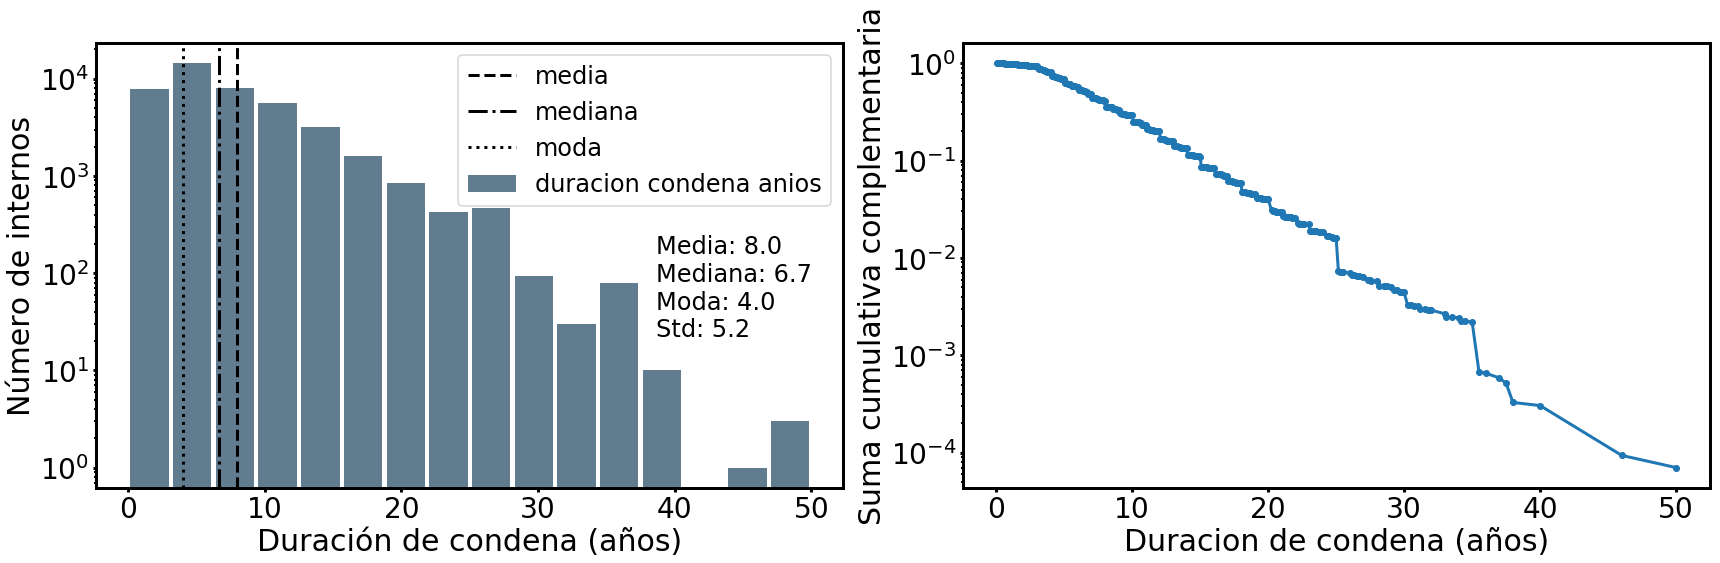
\includegraphics[scale=0.3]{graficos/duracion.png}
	\caption{}
\end{figure}

\subsection{variable3}

\subsection{variable4}

\section{Evolución de variables en el tiempo}
Seleccionar dos variables y graficar cómo fueron cambiando desde 2002 a 2017. Para ello se tiene que utilizar el siguiente conjunto de datos: \url{https://github.com/camporeale/Datos/raw/master/sneep_2002_2017_diplodatos.zip}\\

Las variables elegidas fueron situación legal y participación en programas educativos.

\subsection{Situación legal}

Veamos cómo evoluciona la cantidad de internos condenados y procesados a lo largo de los años, y si nuestro análisis se condice con el de la nota de chequeado: \url{https://chequeado.com/ultimas-noticias/martin-casares-por-primera-vez-en-la-historia-en-2017-el-porcentaje-de-condenados-supero-al-de-procesados/}

\begin{figure}[H]
	\centering
	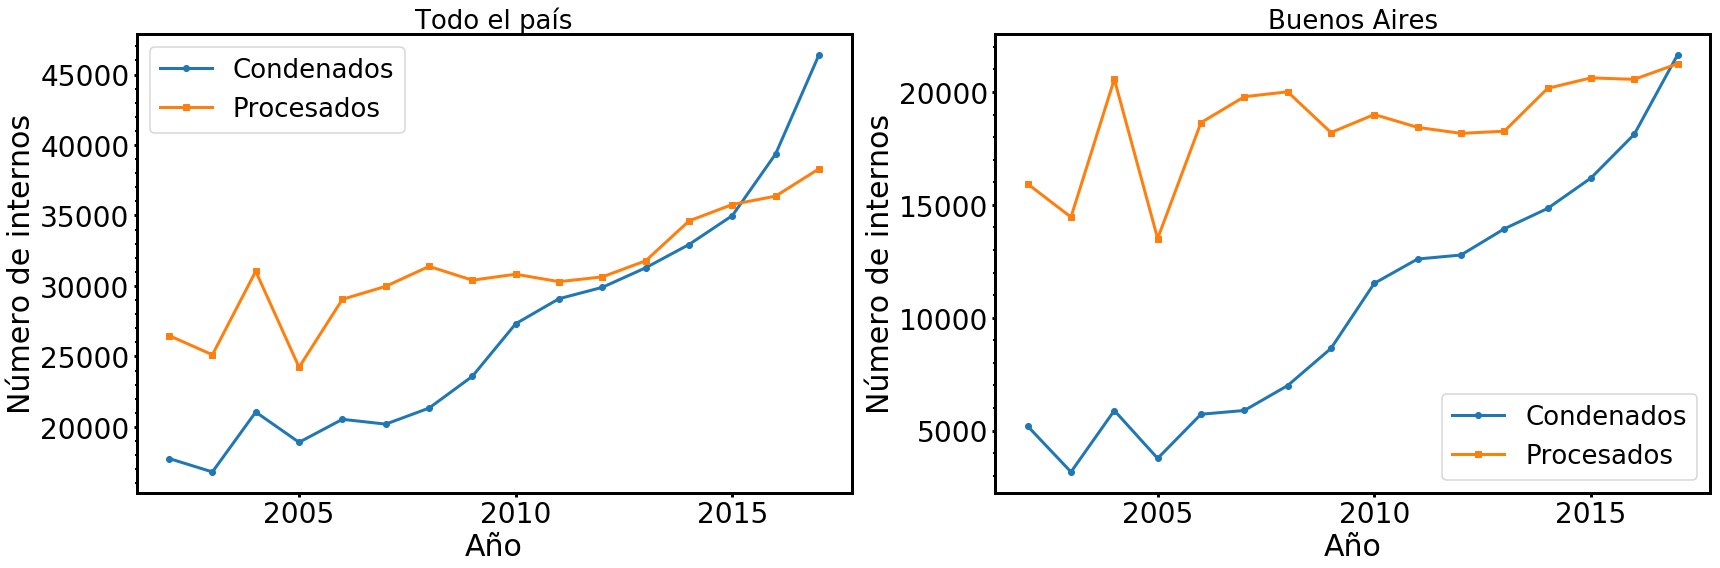
\includegraphics[scale=0.3]{graficos/situacion.png}
	\caption{}
\end{figure}

\begin{figure}[H]
	\centering
	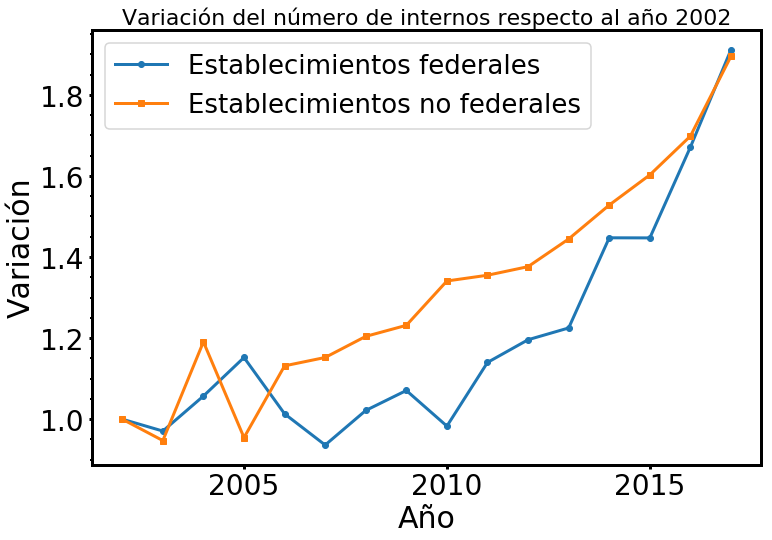
\includegraphics[scale=0.3]{graficos/variacion.png}
	\caption{}
\end{figure}

\subsection{Participación en programas educativos}

Queremos ver cómo varía la proporción de internos que participa en programas educativos a lo largo del tiempo.

\begin{figure}[H]
	\centering
	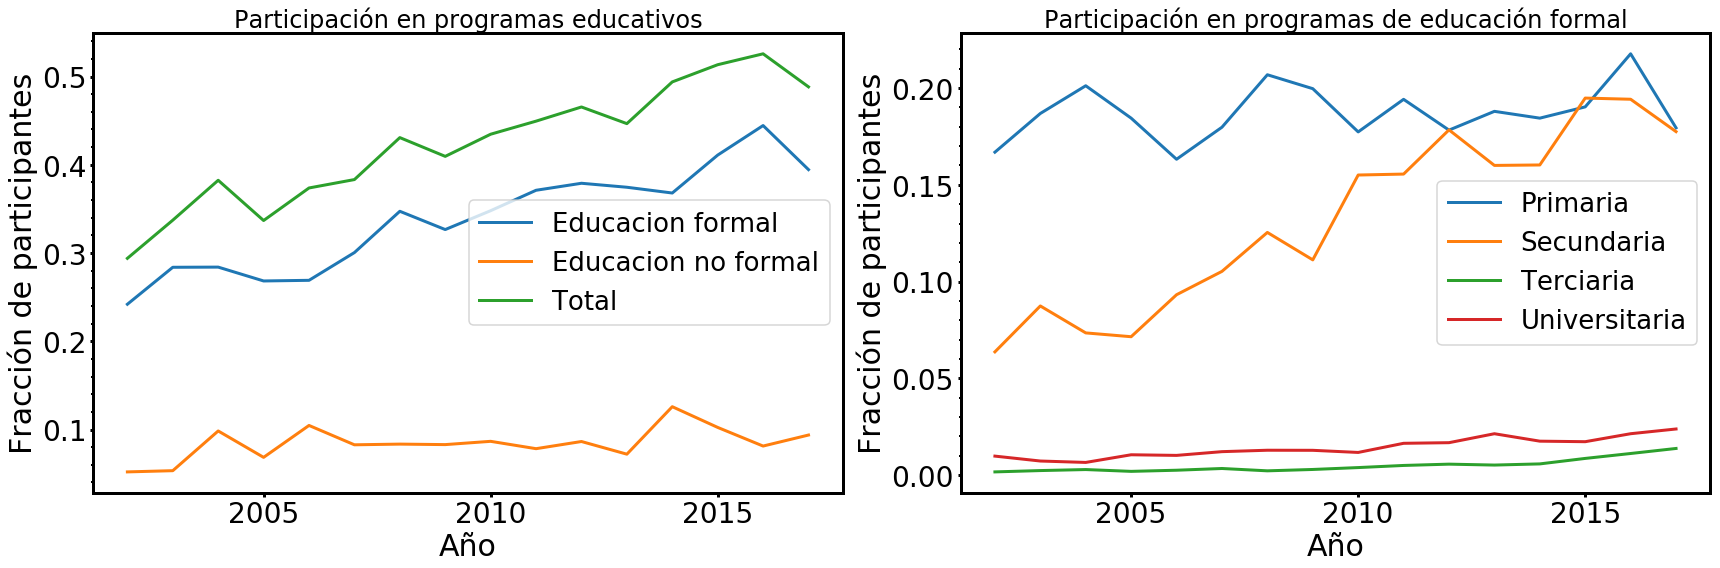
\includegraphics[scale=0.3]{graficos/educacion.png}
	\caption{}
\end{figure}

\section{Análisis de probabilidades condicionales}
Tomar al menos dos pares de variables y realizar un análisis del tipo:

\begin{itemize}
	\item ¿Cuál es la probabilidad de que el interno haya sido lesionado en el último año dado que está en una prisión en Buenos Aires? ¿Y en Córdoba?
	\item ¿Cuál es la probabilidad de que se le otorguen salidas provisorias dado que esté casado/a? ¿Y siendo soltero?
\end{itemize}



\end{document}